\documentclass[
	pages,
	boxes,
	color=RoyalPurple
]{homework}


\usepackage{macros}
\usepackage{tikz}
\usetikzlibrary{quantikz,trees,arrows}
\name{Nate Stemen}
\studentid{20906566}
\email{nate@stemen.email}
\term{Fall 2021}
\course{General Relativity for Cosmology}
\courseid{AMATH 875}

\hwname{Lecture}
\hwnum{2}
\duedate{Thur, Apr 8, 2020 11:59 PM}

\colorlet{Ppink}{WildStrawberry!20}
\newtcbox{\mafbox}[1][]{on line, math upper,
boxsep=4pt, left=0pt,right=0pt,top=0pt,bottom=0pt,
colframe=white,colback=Ppink,
highlight math style={enhanced}}


\makeatletter
\numberwithin{tcb@cnt@prob}{section}
\makeatother


\begin{document}

\setcounter{section}{11}

\begin{problem}
Prove the Kraus representation theorem in the case $\mathcal{H} = \C^D$.
\end{problem}

\begin{solution}
\end{solution}

\begin{problem}
Show that there is a unitary freedom in choosing the set of Kraus operators associated with any fixed unitary acting on an extended Hilbert space. This is connected with the freedom one has in assigning a state to the auxiliary system in the extended Hilbert space.
\end{problem}

\begin{solution}
    When deriving the Kraus operator representation we took the evolution of system $A$ to be
    \begin{equation*}
        \rho_A\to\rho_A' = \tr_B(\mathcal{E}(\rho)) = \tr_B(\hat{U}\rho_A\otimes\rho_B\hat{U}^\dagger)
    \end{equation*}
    and then we explicitly calculated that value in a chosen basis of $\mathcal{H}_B$. That said, there are many bases we could chose to calculate the trace over, and in particular any one is related to another by some unitary operatory $\hat{V}$. Repeating the calculation in a new basis $\qty{\ket{\mu}}$ which is related to the old basis by
    \begin{equation*}
        \ket{l} = \sum_\mu V_{l \mu}\ket{\mu}.
    \end{equation*}
    The Kraus operators we defined $\hat{A}_{kl}\defeq \sqrt{\lambda_l}\qty(\1\otimes\bra{k})\hat{U}\qty(\1\otimes\ket{l})$ can then be rewritten in this new basis.
    \begin{align*}
        \hat{A}_{kl} & =  \sqrt{\lambda_l}\qty(\1\otimes\bra{k})\hat{U}\qty(\1\otimes\ket{l})                                                              \\
                     & =  \sqrt{\lambda_l}\qty(\1\otimes\qty[\sum_\mu \overline{V_{k\mu}}\bra{\mu}])\hat{U}\qty(\1\otimes\qty[\sum_\nu V_{l\nu}\ket{\nu}]) \\
                     & = \sqrt{\lambda_l}\sum_{\mu,\nu}\overline{V_{k\mu}}V_{l\nu}\qty(\1\otimes\bra{\mu})\hat{U}\qty(\1\otimes\ket{\nu})
    \end{align*}
\end{solution}

\problemnumber{4}
\begin{problem}
Generalize the above example of two successive $U_\text{CNOT}$ operations to show that the second transformation can not be modelled by a linear map even when the input state (at time $t = 1$) has no entanglement between systems $A$ and $B$.
\end{problem}

\begin{solution}
    We first lay out the circuit we're working with and the associated states.
    \begin{center}
        \begin{quantikz}
            \slice{$\ket{\psi_0}$} & \qw & \ctrl{1} & \qw\slice{$\ket{\psi_1}$} & \qw & \ctrl{1} & \qw\slice{$\ket{\psi_2}$} & \qw  \\[.5cm]
            & \qw & \targ{}  & \qw                       & \qw & \targ{}  & \qw                       & \qw
        \end{quantikz}
    \end{center}
    Take $\ket{\psi_0} = \qty(a\ket{0} + b\ket{1})\otimes\qty(c\ket{0} + d\ket{1})$ and we first apply a CNOT. % chktex 13
    \begin{align*}
        \ket{\psi_1} & = \hat{U}_\text{CNOT}\ket{\psi_0} = ac\ket{00} + ad\ket{01} + bc\ket{10} + bd\ket{11} \\
                     & = a\ket{0}\otimes(c\ket{0} + d\ket{1}) + b\ket{1}\otimes(c\ket{1} + d\ket{0})
    \end{align*}
    Since $\hat{U}_\text{CNOT}^2 = \1$ we know the final state $\ket{\psi_2}$ is $\ket{\psi_0}$. Now if we look at the evolution of system $B$ alone we have
    \begin{center}
        \tikzstyle{level 1}=[level distance=30mm, sibling distance=30mm]
        \tikzstyle{level 2}=[level distance=40mm]
        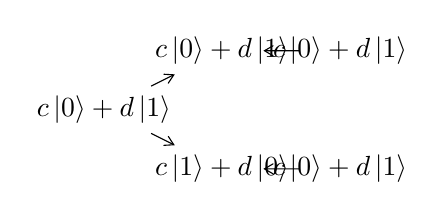
\begin{tikzpicture}[grow=right,->,>=angle 60]
            \node(id){$c\ket{0} + d\ket{1}$}
            child {node {$c\ket{1} + d\ket{0}$}
                    child {node{$c\ket{0} + d\ket{1}$}}
                }
            child {node {$c\ket{0} + d\ket{1}$}
                    child {node{$c\ket{0} + d\ket{1}$}}
                };
        \end{tikzpicture}
    \end{center}
    Not only is the first evolution under a CNOT not even a function, but the second CNOT acts as a swap on one qubit, but the identity on another. If there was a linear map that performed this $N$, then by the top equation $N(c\ket{0} + d\ket{1}) = cN\ket{0} + dN\ket{1} = c\ket{0} + d\ket{1}$ and hence $N$ is the identiy operator $\1$. The second equation, however shows $N(c\ket{1} + d\ket{0}) = cN\ket{1} + dN\ket{0} = c\ket{0} + d\ket{1}$ and hence is the swap. These two operators are clearly not compatible, so it is not possible.

    I'm not sure I've really done what was asked of me here, because of how similar the argument is to in the notes, but the question is somewhat ambiguous.
\end{solution}

\begin{problem}
Find upper and lower bounds on $p$ from the requirement that the depolarizing channel is a CPTP map.
\end{problem}

\begin{solution}
    The Kraus representation theorem tells us that a channel is a CPTP map if and only if it admits an operator sum decomposition which we found in class with the following Kraus operators.
    \begin{align*}
        \hat{A}_{0,0} & = \qty(1 - p + \frac{p}{D^2})^{1/2}\1 & \hat{A}_{a,b} & = \frac{\sqrt{p}}{D}X^a Z^b
    \end{align*}
    To derive bounds on $p$ we need to ensure this \emph{is} a CPTP map and so it must satisfy the completeness relation.
    \begin{align*}
        \1  = \sum_{a, b = 0}^{D-1}\hat{A}_{a,b}^\dagger\hat{A}_{a,b} & = \abs{1 - p + \frac{p  }{D^2}} \1 + \frac{\abs{p}}{D^2}\sum_{a, b = 1}^{D-1}\qty(X^a Z^b)^\dagger X^a Z^b %         \\
        %   & = \abs{1 - p + \frac{p  }{D^2}} \1 + \frac{\abs{p}}{D^2}\sum_{a, b = 1}^{D-1}{Z^\dagger}^b {X^\dagger}^{a} X^a Z^b \\
        %   & = \abs{1 - p + \frac{p  }{D^2}} \1 + \frac{\abs{p}}{D^2}(D - 1)\1
    \end{align*}
    Even without going any further we know that each term must have a positive coefficient since $A^\dagger A \geq 0$ for any operator $A$. The $a, b \neq 0$ term tells us $\abs{p} \geq 0$
    % \begin{align*}

    % \end{align*}
\end{solution}

\setcounter{section}{12}
\problemnumber{2}
\begin{problem}
Determine the full freedom in defining sets of measurement operators $M_{k,j}$ associated with a given POVM $\qty{E_k}$. For example, is the unitary $V$ on $\mathcal{H}_A$ (defined above) the most general map on the output state that is consistent with the Born rule probabilities?
\end{problem}

\begin{solution}
\end{solution}

\setcounter{section}{15}
\problemnumber{1}
\begin{problem}
Assuming that $B_1 = \1_D / \sqrt{D}$ where $\alpha\in\qty{1,\ldots,D^2}$, prove that for any trace-preserving (TP) map $\mathcal{E}$ one has $t(\mathcal{E}) = 1$ and $\va{m} = \va{0}$, and, if $\mathcal{E}$ is a unital map, then $t(\mathcal{E}) = 1$ and $\va{m} = \va{n} = \va{0}$.
\end{problem}

\begin{solution}
    To calculate $t(\mathcal{E})$ or $\mathcal{E}_{1,1}$ which we can calculate with $\mathcal{E}_{\alpha\beta} = \tr(B_\alpha^\dagger\mathcal{E}(B_\beta))$.
    \begin{equation*}
        t(\mathcal{E}) = \mathcal{E}_{11} = \frac{1}{D}\tr(\1_D\mathcal{E}(\1_D)) = \frac{1}{D} \tr(\mathcal{E}(\1_D)) \stackrel{\text{(TP)}}{=} \frac{1}{D}\tr(\1_D) = 1
    \end{equation*}
    Now we want to show $\va{m} = \mathcal{E}_{1\alpha} = \va{0}$ for $\alpha > 1$.
    \begin{equation*}
        \mathcal{E}_{1\alpha} = \frac{1}{\sqrt{D}}\tr(B_1^\dagger\mathcal{E}(P_\alpha)) = \frac{1}{D}\tr(\mathcal{E}(P_\alpha)) \stackrel{\text{(TP)}}{=} \frac{1}{D}\tr(P_\alpha) = 0
    \end{equation*}
    Using the fact that all the Pauli's are traceless, and hence so are the tensor products.

    Now take $\mathcal{E}$ to be unital in addition, and hence we must show $\mathcal{E}_{\alpha 1} = \va{n} = \va{0}$.
    \begin{equation*}
        \mathcal{E}_{\alpha 1} = \frac{1}{D}\tr(P_\alpha^\dagger\mathcal{E}(\1_D)) = \frac{1}{D}\tr(P_\alpha\1_D) = \frac{1}{D}\tr(P_\alpha) = 0
    \end{equation*}
    Thus when $\mathcal{E}$ is both trace preserving and unital it's natural representatation takes the following block form.
    \begin{equation*}
        \mqty[0 & \va{0}^\intercal \\ \va{0} & \vb{R}(\mathcal{E})]
    \end{equation*}
\end{solution}

\end{document}